\section{Anexos}

\subsection{Video del experimento}

Video del experimento con 1M de registros, con y sin índices: \textbf{[enlace al video]}.

En el video se restaura \texttt{dumps/genvar\_\allowbreak{}1000000.dump}, se ejecutan las consultas de \texttt{07\_\allowbreak{}consultas.sql}
sin índices con \texttt{\textbackslash timing on}, se crean los índices con \texttt{08\_\allowbreak{}indices.sql} y se vuelven a
ejecutar las mismas consultas.

\subsection{MVP web}

Como punto extra se desarrolló una aplicación web en Python (Flask) conectada directamente a la base de datos
PostgreSQL (carpeta \texttt{web/}). Permite:

\begin{itemize}
  \item Ejecutar las consultas C1 a C8 con sus parámetros y ver el resultado, el tiempo, el SQL y el plan de ejecución.
        Las cinco consultas del experimento usan el mismo SQL de la Sección~5.1.2.
  \item Ver la ficha de un donante con sus muestras y su reporte clínico (\texttt{fn\_\allowbreak{}reporte\_\allowbreak{}clinico}).
  \item Registrar donantes y muestras, reclasificar anotaciones y revocar consentimientos con los procedimientos
        almacenados. Cuando una operación viola una regla, la aplicación muestra el error que lanza el trigger
        (por ejemplo, T3 al registrar una muestra de un donante sin consentimiento).
  \item Borrar y crear los índices finales y comparar los tiempos de las cinco consultas del experimento.
  \item Actuar como cada tipo de usuario (\texttt{SET ROLE}) para comprobar los permisos de la Sección~4.4.
\end{itemize}

Se ejecuta con \texttt{pip install -r web/requirements.txt} y \texttt{python web/app.py}, y se abre en
\texttt{http://localhost:5000}.

\begin{figure}[H]
\centering
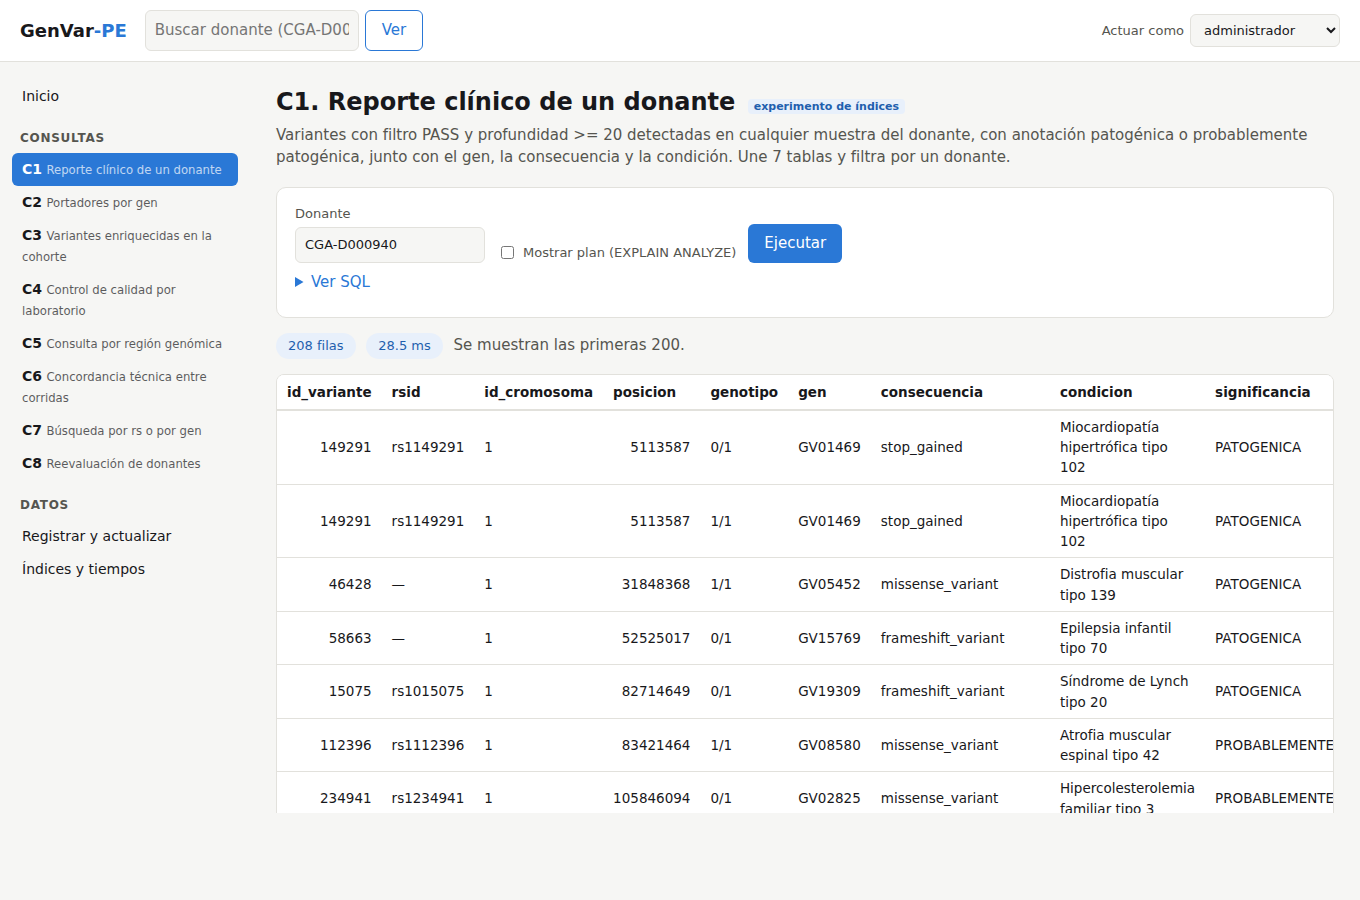
\includegraphics[width=0.9\textwidth]{fig/web_consulta.png}
\caption{MVP web: ejecución de la consulta C1 con 1M de genotipos.}
\end{figure}

\begin{figure}[H]
\centering
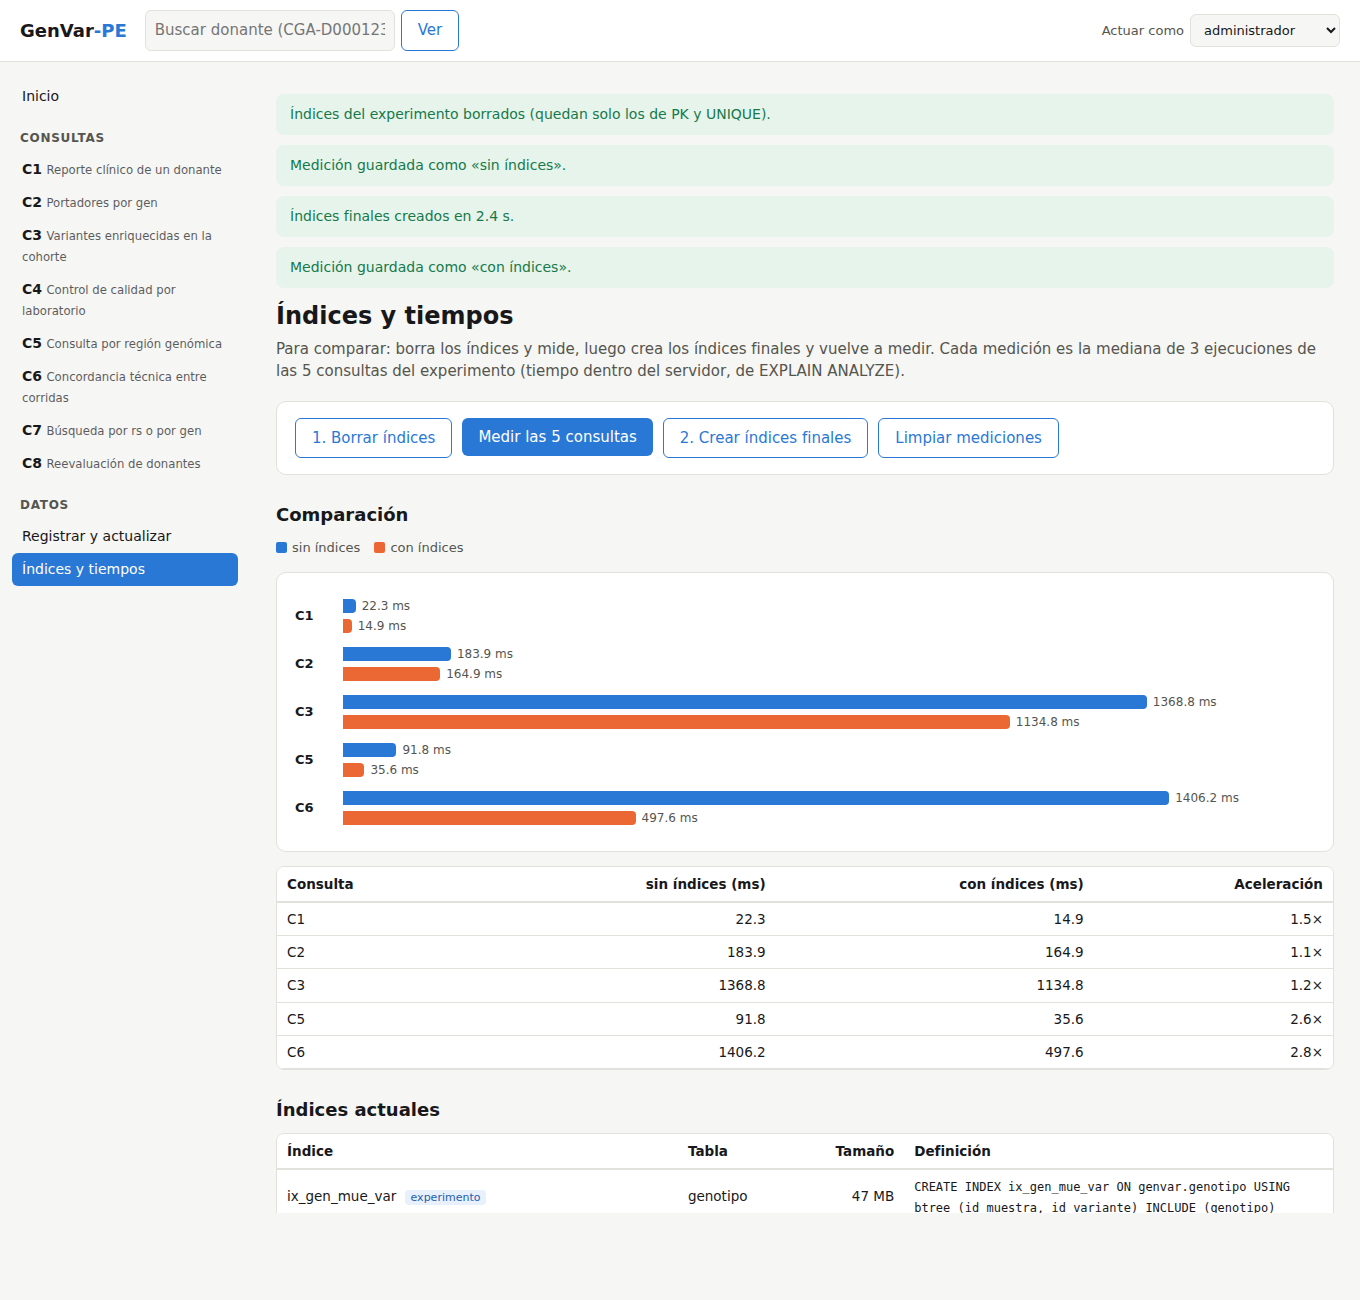
\includegraphics[width=0.9\textwidth]{fig/web_indices.png}
\caption{MVP web: comparación de tiempos sin índices y con los índices finales.}
\end{figure}

\subsection{Archivos entregados}

\begin{table}[H]
\centering\small
\begin{tabular}{@{}l>{\raggedright\arraybackslash}p{9.5cm}@{}}
\toprule
Ruta & Contenido \\
\midrule
\texttt{sql/} & Scripts 01 a 09 (Sección 4 y 5) \\
\texttt{dumps/} & Los cuatro dumps: \texttt{genvar\_\allowbreak{}1000.dump}, \texttt{genvar\_\allowbreak{}10000.dump}, \texttt{genvar\_\allowbreak{}100000.dump}, \texttt{genvar\_\allowbreak{}1000000.dump} \\
\texttt{exp/consultas.py} & Consultas y planes de índices (fuente única) \\
\texttt{exp/experimento.py} & Script que genera los escenarios y mide los tiempos \\
\texttt{exp/resultados.json} & Todas las mediciones (las 7 repeticiones, planes usados y filas) \\
\texttt{exp/graficos.py} & Genera las figuras de la Sección 5.6 \\
\texttt{exp/salida\_\allowbreak{}pruebas.txt} & Salida de \texttt{09\_\allowbreak{}pruebas.sql} \\
\texttt{web/} & MVP web (Flask): \texttt{app.py}, plantillas y \texttt{LEEME.md} con las instrucciones \\
\bottomrule
\end{tabular}
\caption{Contenido del repositorio del proyecto.}
\end{table}

\subsection{Cómo reproducir el experimento}

\begin{lstlisting}[language=bash]
createdb genvar
for f in 01_esquema 02_vistas 03_procedimientos 04_triggers 05_roles; do
  psql -d genvar -f sql/$f.sql
done
pip install psycopg2-binary matplotlib
python3 exp/experimento.py --reps 7     # genera los 4 escenarios, los dumps y resultados.json
python3 exp/graficos.py                 # genera fig/*.png
psql -d genvar -f sql/08_indices.sql    # deja los índices finales
psql -d genvar -f sql/09_pruebas.sql    # pruebas de triggers y procedimientos
\end{lstlisting}
